\documentclass[11pt]{beamer}
\usepackage[utf8]{inputenc}
\usepackage[T1]{fontenc}
\usepackage{lmodern}
\usepackage{amsmath}
\usepackage{amsfonts}
\usepackage{amssymb}
\usepackage{graphicx}
\usetheme{cambridgeUS}
\usepackage[longnamesfirst]{natbib} 
\usepackage{caption}
\DeclareCaptionFormat{citation}{%
	\ifx\captioncitation\relax\relax\else
	\captioncitation\par
	\fi
	#1#2#3\par}
\newcommand*\setcaptioncitation[1]{\def\captioncitation{\textit{Source:}~#1}}
\let\captioncitation\relax
\captionsetup{format=citation,justification=centering}
\usepackage {subcaption}
\usepackage{CJKutf8}
%代码设置
\usepackage{verbatim}
\usepackage{cprotect}
\usepackage{listings}
\usepackage{color}
\usepackage{xcolor}
\usepackage{showexpl} 
%\usepackage{enumitem}
\lstloadlanguages{[LaTeX]Tex} 
\lstset{ %
	language=TeX,                % the language of the code
	basicstyle=\footnotesize,           % the size of the fonts that are used for the code
	numbers=left,                   % where to put the line-numbers
	numberstyle=\tiny\color{black},  % the style that is used for the line-numbers
	stepnumber=1,                   % the step between two line-numbers. If it's 1, each line 
	% will be numbered
	%numbersep=5pt,                  % how far the line-numbers are from the code
	backgroundcolor=\color[RGB]{229, 231, 233},      % choose the background color. You must add \usepackage{color}
	showspaces=false,               % show spaces adding particular underscores
	showstringspaces=false,         % underline spaces within strings
	showtabs=false,                 % show tabs within strings adding particular underscores
	frame=single,                   % adds a frame around the code
	frameround=ffff
	rulecolor=\color{black},        % if not set, the frame-color may be changed on line-breaks within not-black text (e.g. commens (green here))
	tabsize=2,                      % sets default tabsize to 0 spaces
	captionpos=b,                   % sets the caption-position to bottom
	breaklines=true,                % sets automatic line breaking
	breakatwhitespace=false,        % sets if automatic breaks should only happen at whitespace
	title=\lstname,                 % show the filename of files included with \lstinputlisting;
	% also try caption instead of title
	keywordstyle=\color{blue},          % keyword style
	commentstyle=\color[RGB]{17,122,101},       % comment style
	%	stringstyle=\color{mauve},         % string literal style
	escapeinside={\%*}{*)},            % if you want to add LaTeX within your code
	morekeywords={*,...}               % if you want to add more keywords to the set
}

\definecolor{myred}{RGB}{231, 76, 60}
\setbeamertemplate{caption}[numbered]

\setbeamercolor{section name}{fg=white}

\makeatletter
\setbeamertemplate{section page}
{
	\begingroup
	\centering
	%    {\usebeamerfont{section name}\usebeamercolor[fg]{section name}\sectionname~\insertsectionnumber}
	\vskip1em\par
	\begin{beamercolorbox}[sep=12pt,center,colsep=-4bp,rounded=true,shadow=\beamer@themerounded@shadow]{section title}
		\usebeamerfont{section title}\insertsection\par
	\end{beamercolorbox}
	\endgroup
}
\makeatother
\begin{document}
	
	\begin{CJK*}{UTF8}{gkai}
		
	\author[LC Meng]{Lingchao Meng}
	\title[LaTeX Tutorial]{\LaTeX\ Tutorial}
	%\subtitle{}
	%\logo{}
	\institute[SE, PKU]{School of Economics\\Peking University}
	%\date{}
	%\subject{}
	%\setbeamercovered{transparent}
	%\setbeamertemplate{navigation symbols}{}
\begin{frame}
    \maketitle
\end{frame}

\begin{frame}
	This is  just a beginners guide to writing documents in \LaTeX\ without prior knowledge of \LaTeX. This slide is designed for the \LaTeX\ workshop at School of Economics, Peking University.
\end{frame}

\begin{frame}
	This file and some other materials can be download from my GitHub repository: \underline{https://github.com/MengLingchao/LaTex\_tutorial}. \\Please feel free to download and use it.\\
	If you want, you can also star it!
	\begin{figure}
		\centering
		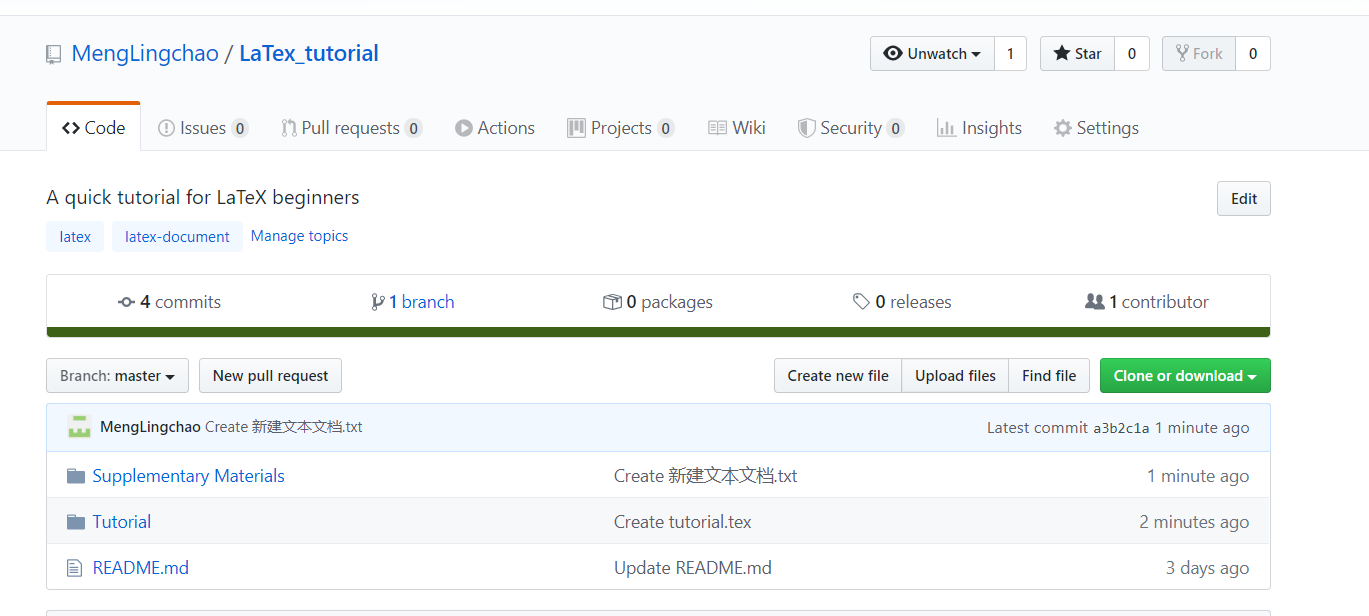
\includegraphics[width=0.7\linewidth]{figs/GitHub}
		\caption{GitHub Repository}
		\label{fig:github}
	\end{figure}
	
\end{frame}

\begin{frame}{Outline}
	\tableofcontents
\end{frame}

\section{Introduction}
\begin{frame}
	\sectionpage
\end{frame}

\begin{frame}[fragile]{What's \LaTeX?}
\LaTeX\ (pronounced either “Lay-tech” or “Lah-tech”) 
	\begin{itemize}
		\item is based on Tex, a typesetting system designed by Donald Knuth in 1978 for high quality digital typesetting.
		\item is a \textit{typesetting system} and \textit{programming language}, not a \textit{word processor}.
	\end{itemize}

\vskip 0.25cm
\begin{LTXexample}[caption={the typesetting nature of \LaTeX}]
This is \textbf{my} \emph{first} document prepared in \LaTeX. I \underline{typed} it on \today.
\end{LTXexample} 
\end{frame}

\begin{frame}{Why \LaTeX?}
\begin{itemize}
	\item Donald Knuth says that his aim in creating TEX is to beautifully
	typeset \textit{technical documents} especially those \textit{containing a lot of Mathematics}.
	\item Most English journals have their own \LaTeX\ template.
	\item Even for ordinary text, \LaTeX\ is also a good choice.
\end{itemize}
\end{frame}

\begin{frame}{Installation}
	On Windows, users have two main choices of TeX system to install: \alert{TeX Live} or \alert{MiKTeX}. I highly recommend Tex Live for the following reasons
	\begin{itemize}
		\item The standard installer for MiKTeX installs 'just the basics' and uses on-the-fly installation for anything else you need; the standard install for TeX Live is 'everything' (about 4.5 Gb!).
		\item Real-time updates.
		\item Faster compilation (especially in case of graphics files)
	\end{itemize}
\end{frame}

\begin{frame}{Installation}
There are many different editors of \LaTeX.
\begin{itemize}
\item professional \LaTeX\ editors, such as TeXstudio, TeXwork.
\item edit \LaTeX files using Vim, Sublime Text, Visual Code, etc.
\item For more comparison of \LaTeX, you can refer to https://en.wikipedia.org/wiki/Comparison\_of\_TeX\_editors
\end{itemize}
 \vskip 0.75cm

Recommend Tex Live with TexStudio, you can refer to https://blog.csdn.net/zywhehe/article/details/83113214. 
\end{frame}

\begin{frame}{Installation}
 \begin{figure}
 	\centering
 	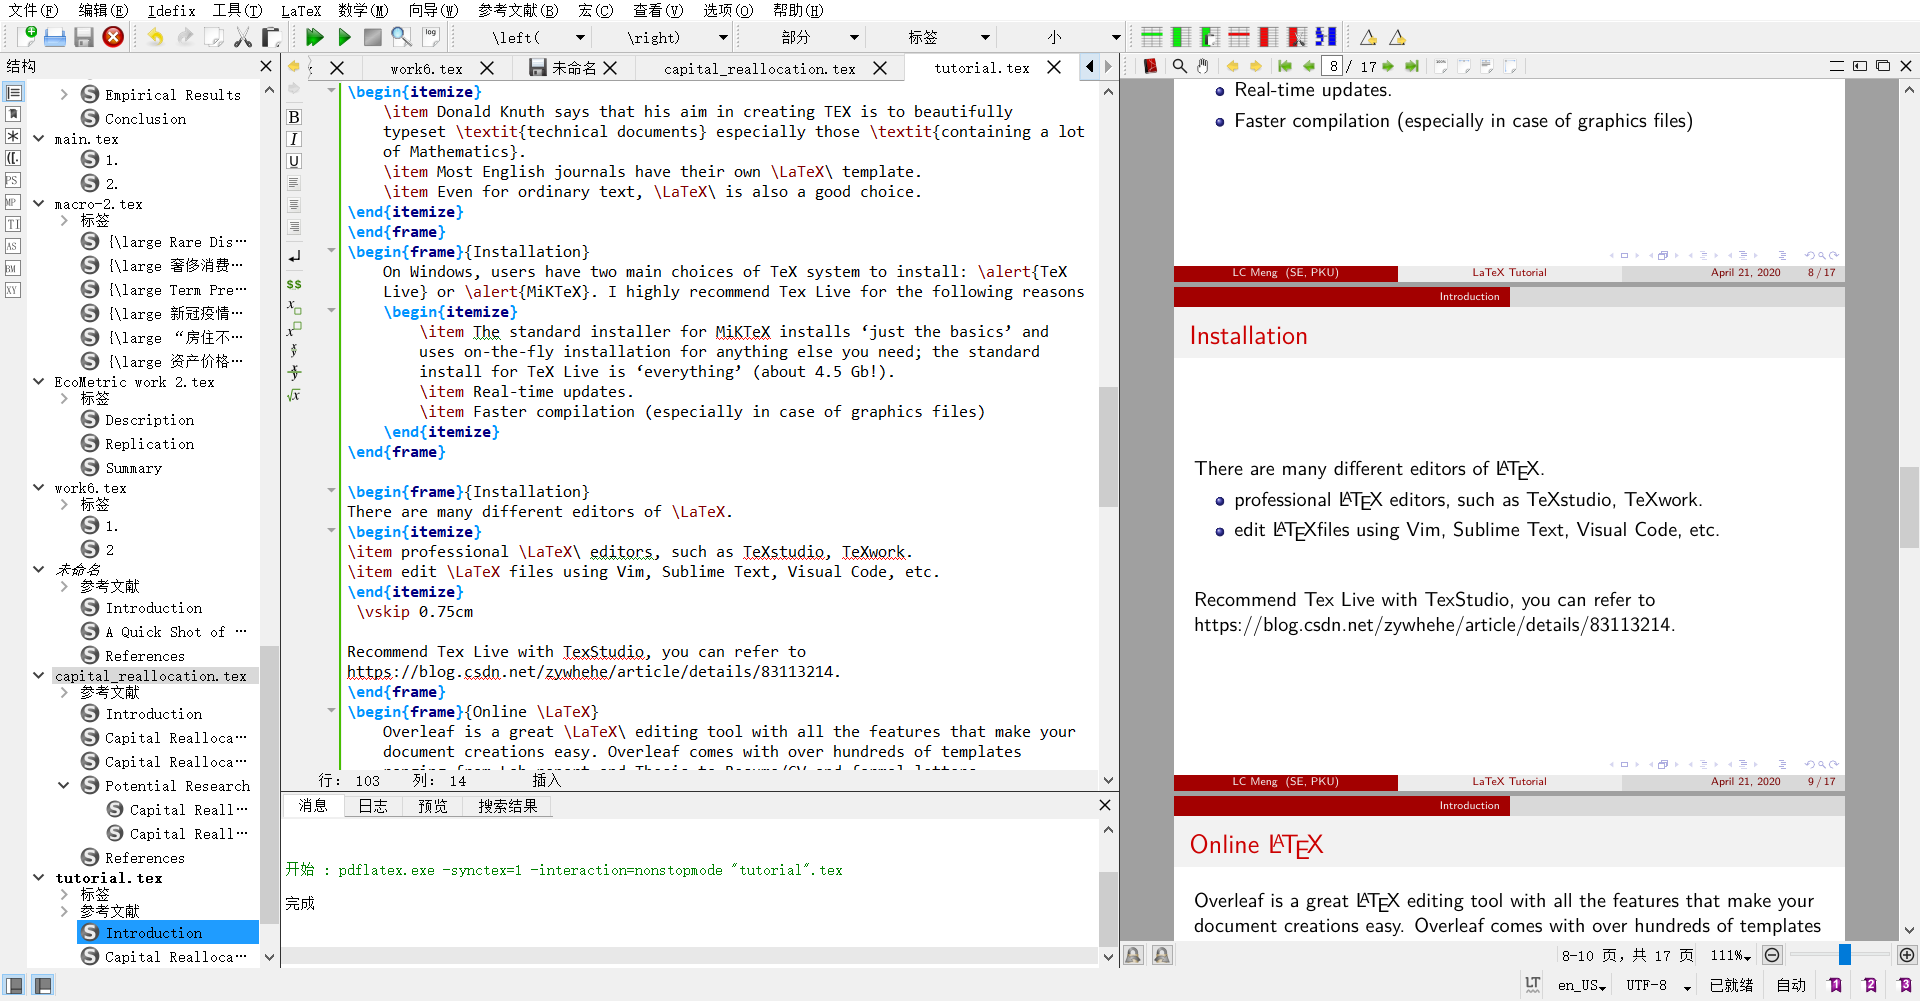
\includegraphics[width=0.85\linewidth]{figs/TeXstudio}
 	\caption{TeXstudio}
 	\label{fig:texstudio}
 \end{figure}
 
\end{frame}
\begin{frame}{Online \LaTeX}
	
	Overleaf(https://www.overleaf.com/) is a great \LaTeX\ editing tool with all the features that make your document creations easy. Overleaf comes with over hundreds of templates ranging from Lab report and Thesis to Resume/CV and formal letters. 
\begin{figure}
	\centering
	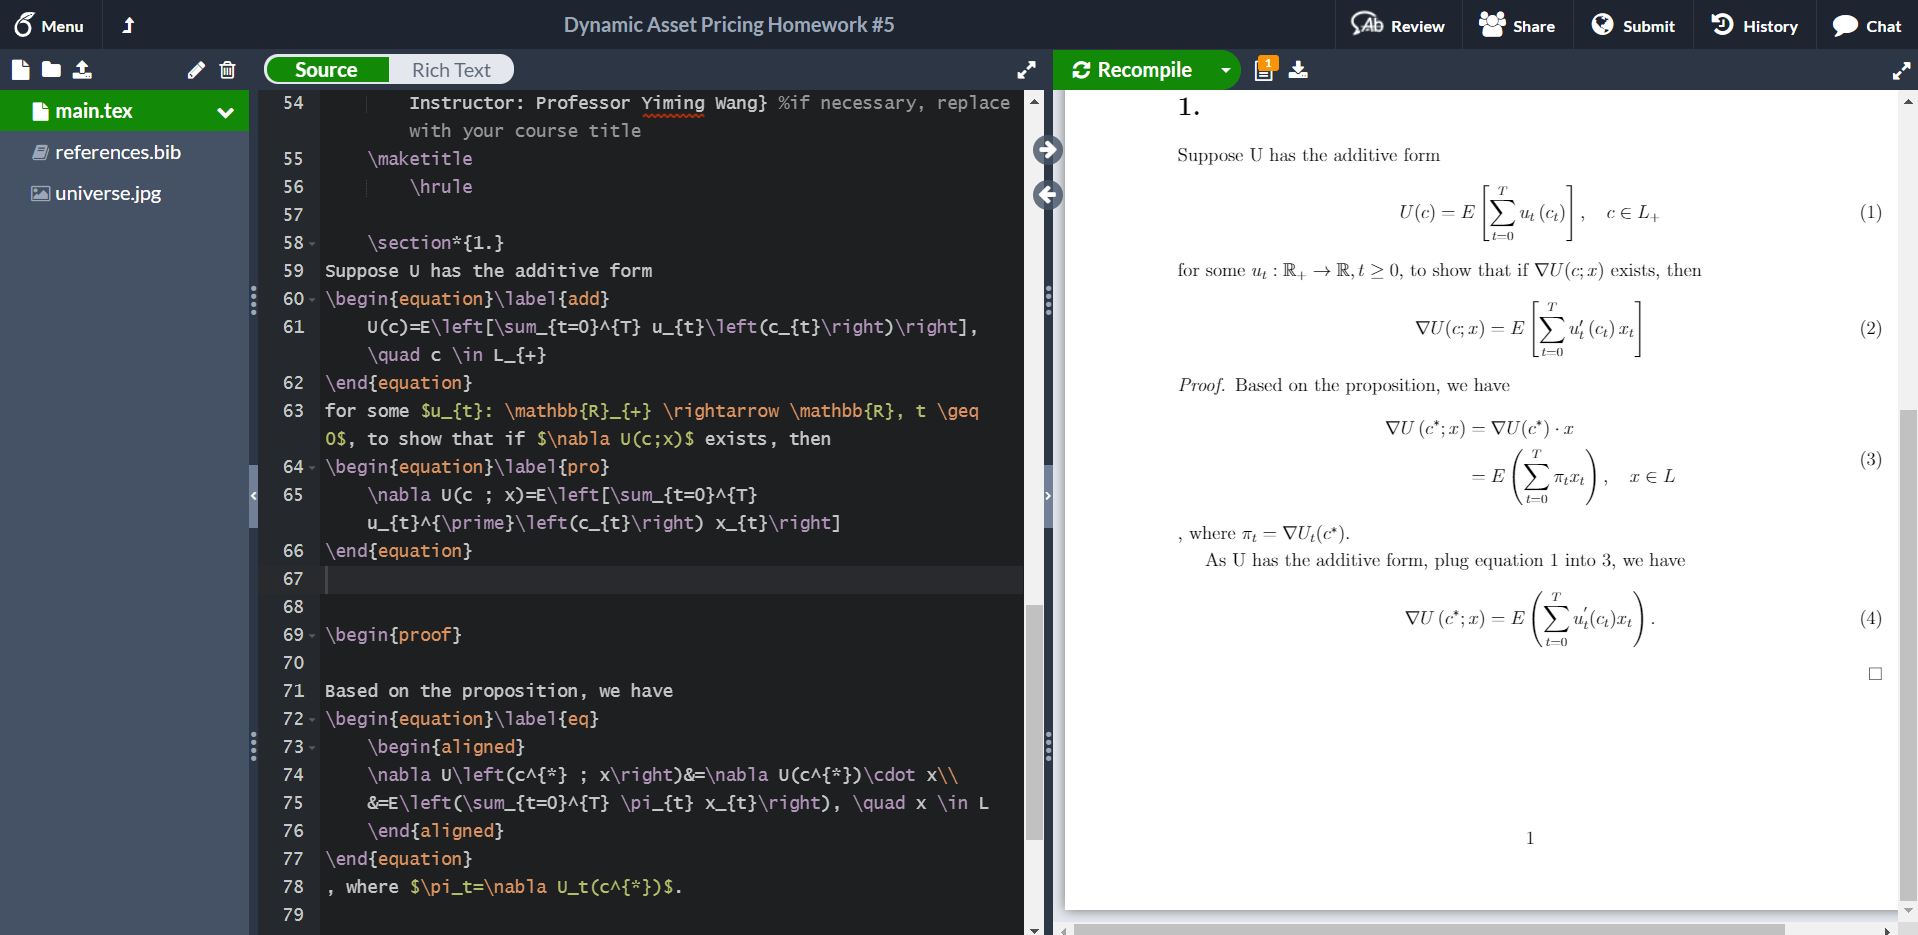
\includegraphics[width=0.7\linewidth]{figs/overleaf}
	\caption{Overleaf website}
	\label{fig:overleaf}
\end{figure}
\end{frame}


\section{\LaTeX\ Basic}


\begin{frame}
	\sectionpage
\end{frame}


\begin{frame}[fragile]{The basic structure of a \LaTeX\ file}
	\begin{enumerate}
		\item The \textit{documentclass} command: define the property of the file
		\begin{itemize}
			\item article, beamer, report, thesis, letter, book
		\end{itemize}
		\item Preamble
		\begin{itemize}
			\cprotect\item include the packages: \verb+\usepackage{package}+
			\item format the article.
		\end{itemize}
		\item Begin and end of the document: the main body of the file.
	\end{enumerate}
\vskip 0.5cm
	\begin{lstlisting}
	\documentclass[options]{article}
	Preamble (for LATEX commands only)
	\begin{document}
	Document text (text with embedded LATEX commands)
	\end{document}
	\end{lstlisting}
\end{frame}


\begin{frame}[fragile]{Document Structure}
	\LaTeX\ can organize, number, and index chapters and sections of document. There are up to 7 levels of depth for defining sections depending on the document class
	\begin{itemize}
		\cprotect\item \verb+\part{title}+
		\cprotect\item \verb+\chapter{title}+
		\cprotect\item \verb+\section{title}+
		\cprotect\item \verb+\subsection{title}+
		\cprotect\item \verb+\subsubsection{title}+
		\cprotect\item \verb+\paragraph{title}+
		\cprotect\item \verb+\subparagraph{title}+
	\end{itemize}
\end{frame}


\begin{frame}[fragile]{\LaTeX\ vocabulary}
	\begin{itemize}
		\cprotect\item \textbf{Commands}: produce text or space, like \verb+\textit{it}+.
		\cprotect\item \textbf{Declarations}: affect the following text, like \verb+\Large+ or \verb+{\Large }+.
		\cprotect\item \textbf{Environments}:receive special processing and are defined by \verb+\begin{name} ... \end{name}+.
		\cprotect\item \textbf{Mandatory arguments}: are included in braces, like \verb+\hspace{2in}+.
		\cprotect\item \textbf{Optional arguments}: are enclosed in brackets [ ], like \verb+\documentclass[11pt]{article}+.
		\item \textbf{*}: indicates a variation on a command or environment.
	\end{itemize}
\end{frame}

\begin{frame}{A little sample}
	\begin{center}
		\alert{{\Large See the simple sample!}}
	\end{center}
\end{frame}

\section{Basic Typesetting}

\begin{frame}
	\sectionpage
\end{frame}

\begin{frame}[fragile]{Basic Typesetting}
	\begin{itemize}
		\item Simply enter your content in most times, just like using word or txt.
		\cprotect\item When you need to start a new paragraph, add \verb+\par+ in the end or empty one line between two paragraphs.
	\end{itemize}

\vskip 0.5cm
\begin{LTXexample}[caption={new paragraph}]
The first paragraph.\par
The second paragraph.

The third paragraph.
\end{LTXexample}
\end{frame}


\begin{frame}[fragile]{Font effects}
There are \LaTeX\ commands for a variety of font effects:
\begin{LTXexample}[caption={Font effects}]
\textbf{hello world}

\textit{hello wolld}

\underline{hello world}

\textsc{hello world}

\textrm{hello world}
\end{LTXexample}
\end{frame}



 \begin{frame}[fragile]{Colored text}
	\begin{itemize}
		\cprotect\item Include the xcolor package in the preamble by \verb+\usepackage{xcolor}+.
		\cprotect\item Also can define customized color, such as \verb+\definecolor{myred}{RGB}{231, 76, 60}+.
	\end{itemize}

\vskip 1cm

\begin{LTXexample}[caption={Colored text}]
\textcolor{red}{Red}
\textcolor{gray}{Gray}
\textcolor{myred}{Myred}
\end{LTXexample}
\end{frame}


 \begin{frame}[fragile]{Font size}
\begin{itemize}
	\item The global font size can be set by the documentclass option.
	\item The local font size can be changed by the following commands.
\end{itemize}
\begin{LTXexample}[caption={Font size}]
{\tiny tiny}\\
{\scriptsize scriptsize}\\
{\footnotesize footnotesize}\\
{\small small}\\
{\normalsize normalsize}\\
{\large large}\\
{\Large Large}\\
{\LARGE LARGE}\\
{\huge huge}\\
{\Huge Huge}
\end{LTXexample}
\end{frame}

 \begin{frame}[fragile]{Lists}
 	\begin{itemize}
 		\cprotect\item \LaTeX\ supports two types of lists: \textit{enumerate} produces numbered lists, while \textit{itemize} is for bulleted lists. Each list item is defined by \verb+\item+. Lists can be nested to produce sub-lists.
 	\end{itemize}

\begin{LTXexample}[caption={Lists}]
\begin{enumerate}
	\item First thing
	\item Second thing
	\begin{itemize}
		\item A sub-thing
		\item[-] Another sub-thing
	\end{itemize}
	\item[(3)] Third thing
\end{enumerate}
\end{LTXexample}
\end{frame}

 \begin{frame}[fragile]{Comments and Spacing}
	\begin{itemize}
		\cprotect\item \LaTeX\ Comments are created using \%. When \LaTeX\ encounters a \% character while	processing a .tex file, it ignores the rest of the line.
		\item Multiple consecutive spaces in\LaTeX\ are treated as a single space. Several empty lines are treated as one empty line.
		\cprotect\item Use \verb*+\ + to produce more space and \verb+\vspace{length}+ to produce vertical space.
	\end{itemize}
	
\begin{LTXexample}[caption={Comments and Spacing}]
%comments 1
The following is comments 2. % comments 2

more space in line  like \ \ \ ahh.


more vertical space like following.

\vspace{0.5in}

third paragraph.
\end{LTXexample}
\end{frame}

\begin{frame}[fragile]{Special characters}
\begin{LTXexample}[caption={Special characters}]
\# \$ \% \^{} \& \_ \{ \} \~{} \textbackslash
\end{LTXexample}
\end{frame}

\section{Equations}
\begin{frame}
	\sectionpage
\end{frame}

\begin{frame}[fragile]{Mathematical modes}
	\LaTeX\ allows two writing modes for mathematical expressions: the \textit{inline mode} and the \textit{display mode}. The first one is used to write formulas that are part of a text. The second one is used to write expressions that are not part of a text or paragraph, and are therefore put on separate lines.
	\begin{itemize}
		\cprotect\item Inline mode: use \verb|$equation$| or \verb|\(equation\)|
		\cprotect\item Display mode: use \verb|$$equation$$| or \verb|\[equation\]|
	\end{itemize}
\begin{LTXexample}[caption={equations}]
Inline mode: $a=b+c$ or \(a=b+c\)

Display mode:
\[a=b+c\]
$$a=b+c$$
\end{LTXexample}
\end{frame}

\begin{frame}[fragile]{Equation Environment}
	\begin{itemize}
		\item Another useful mode is the equation environment, which support the numbered equation and the reference.
		\cprotect\item The reference can achieved through \verb+\label{}+ and \verb+\ref{}+. The reference of the equation, table and figure are all the same.
	\end{itemize}
	
	
\begin{LTXexample}[caption={equation environment}]
An example 
\begin{equation}\label{eq:myeq}
E=MC^2
\end{equation}
Equation \ref{eq:myeq} is mass-energy equivalence.
\end{LTXexample}	 
\end{frame}

\begin{frame}[fragile]{Subscripts and Superscripts}
Subscripts and superscripts are written using the symbols \^{} and \_.
	
\vskip 1.5cm
\begin{LTXexample}[caption={subscripts and superscripts}]
\[a_1^2=b_1^2+c_1^2\]
\[a_mn^2=b_mn^2\]
\[a_{mn}^2=b_{mn}^2\]
\end{LTXexample}	 
\end{frame}


\begin{frame}[fragile]{Fractions}
	\begin{itemize}
		\item To enable the fraction, you need to include the \textit{amsmath} package, a powerful math package.
		\cprotect\item \verb+\frac{numerator}{denominator}+.
	\end{itemize}
	
	\vskip 1cm
\begin{LTXexample}[caption={fractions}]
\[a_1 = \frac{b_1}{c_1}\]
\[a_1 = \frac{b_1}{c_1} mn\]
\end{LTXexample}	 
\end{frame}

\begin{frame}[fragile]{Brackets and Parentheses}
	\begin{itemize}
		\cprotect\item Use to \verb+\left+ and \verb+\right+ command to set dynamically resized brackets and parentheses.
		\cprotect\item Even if you are using only one bracket, both commands are mandatory.
	\end{itemize}

	\vskip 0.5cm
	\begin{LTXexample}[caption={brackets and parentheses}]
\[U_t=\left((1-\delta)\frac{A}{C}+\delta B\right)^{\frac{1}{1-\sigma}}\]
\[U_t=((1-\delta)\frac{A}{C}+\delta B)^{\frac{1}{1-\sigma}}\]
\[\left(A\right.\]
	\end{LTXexample}	 
\end{frame}

\begin{frame}[fragile]{Aligning equations}
	\begin{itemize}
		\cprotect\item Amsmath package and \verb+\begin{aligned}...\end{aligned}+ environment.
	\end{itemize}
	
	\vskip 0.5cm
\begin{LTXexample}[caption={aligning equations}]
\begin{equation}
\begin{aligned}
\frac{\partial U_t}{\partial A}&=(1-\delta)U_t^{\frac{1}{1-\sigma^{-1}}-1}A^{-\sigma^{-1}}\\
\frac{\partial U_t}{\partial B}&=\delta U_t^{\frac{1}{1-\sigma^{-1}}-1}B^{-\sigma^{-1}}
\end{aligned}
\end{equation}
\end{LTXexample}	 
\end{frame}




\begin{frame}[fragile]{Special symbols}
	\begin{itemize}
		\cprotect\item Integrals, sums and limits.
		\cprotect\item Greek letters.
		\cprotect\item math symbols.
	\end{itemize}
	
	\begin{LTXexample}[caption={special symbols}]
		\[\alpha\]
		\[\beta\]
		\[\int_{a}^{b} x^2 dx\]
		\[\lim_{x\to\infty} f(x)\]
		\[\uparrow\rightarrow\downarrow\leftarrow\]
	\end{LTXexample}	 
\end{frame}


\begin{frame}[fragile]{Special symbols}
	Some trickier equations(not just math)
	
	\begin{LTXexample}[caption={special symbols}]
		\begin{equation}\begin{aligned}
		\oint \mathbf{B} \cdot d \mathbf{S} &=\mu_{0} \epsilon_{0} \frac{d \Phi_{E}}{d t}+\mu_{0} i_{e n c} \\
		k &=A e^{-E_{A} / R T} \\
		K_{a} &=\frac{\left[\mathrm{H}_{3} 0^{+}\right]\left[\mathrm{A}^{-}\right]}{[\mathrm{HA}]} \\
		V &=\left(\bigoplus_{\lambda \in \operatorname{Sec}(T)} V^{(\lambda)}\right) \oplus V
		\end{aligned}\end{equation}
	\end{LTXexample}	 
\end{frame}


\begin{frame}[fragile]{Special symbols}
	Some supplementary material
	\begin{itemize}
		\cprotect\item Latex mathematical symbols.pdf
		\cprotect\item The great, big list of latex symbols.pdf
	\end{itemize}
	
	An online website
	\begin{itemize}
		\item https://www.codecogs.com/latex/eqneditor.php?lang=zh-cn
	\end{itemize}
	\begin{figure}
		\centering
		\includegraphics[width=0.7\linewidth]{"figs/online equation editor"}
		\caption{Online Equation Editor}
		\label{fig:online-equation-editor}
	\end{figure}
	
\end{frame}


\section{Tables and Figures}
\begin{frame}
	\sectionpage
\end{frame}

\begin{frame}[fragile]{Figures}
	\begin{itemize}
		\cprotect\item First include the \textit{graphicx} package.
		\cprotect\item Images should be EPS, PDF, PNG, JPEG or GIF files.
	\end{itemize}
	
	\begin{LTXexample}[caption={special symbols}]
\begin{figure}[h]
	\centering
	\includegraphics[width=0.7\linewidth]{"figs/new york"}
	\caption{new york}
	\label{fig:new-york}
\end{figure}

	\end{LTXexample}	 
\end{frame}

\begin{frame}[fragile]{Figures}

	\begin{enumerate}
		\item \textbf{[h]} is the placement specifier. put the figure approximately here.
		\begin{itemize}
			\item Other options are \textbf{t}(at the top of the page), \textbf{b}(at the bottom of the page) and \textbf{p}(on a separate page for figures).
		\end{itemize}
	\cprotect\item \verb+\centering+ centres the image on the page, if not used images are left-aligned	by default.
	\cprotect\item \verb+includegraphics{...}+ is the command that actually puts the image in your document. The image file should be saved in the same folder as the .tex file.
    	\cprotect\item \verb+[width=0.7\textwidth]+. is an optional command that specifies the width of the picture in this case the same width as the text. The width could also be given in centimeters (cm). 
    	\cprotect\item \verb+\label{...}+  creates a label to allow you to refer to the table or figure in your text.
	\end{enumerate}	 
\end{frame}

\begin{frame}[fragile]{Figures}
	
	\begin{enumerate}
		\item \textbf{[h]} is the placement specifier. put the figure approximately here.
		\begin{itemize}
			\item Other options are \textbf{t}(at the top of the page), \textbf{b}(at the bottom of the page) and \textbf{p}(on a separate page for figures).
		\end{itemize}
		\cprotect\item \verb+\centering+ centres the image on the page, if not used images are left-aligned	by default.
		\cprotect\item \verb+\label{...}+  creates a label to allow you to refer to the table or figure in your text.

	\end{enumerate}	 
\end{frame}

\begin{frame}[fragile]{Tables}
	Tablular environment is used to typeset basic tables.
	\begin{enumerate}
		\cprotect\item The braces after \verb+\begin{tabular}+ defines the columns.
		\begin{itemize}
			\item l for a column of left-aligned text.
			\item r for a column of right-aligned text.
			\item c for a column of center-aligned text.
			\item $|$ for a vertical line.
		\end{itemize}
	\end{enumerate}

	\begin{LTXexample}[caption={Simple tables}]
	\begin{tabular}{|rc}
		Apples & Green \\
		\hline
		Strawberries & Red \\
		\cline{1-1}
		Oranges & Orange \\
	\end{tabular}	
		\end{LTXexample}
\end{frame}

\begin{frame}[fragile]{Tables}
	Tablular environment is used to typeset basic tables.
	\begin{enumerate}
		\cprotect\item The table data follows the \verb+\begin+ command:
		\begin{itemize}
			\item $\&$ is placed between columns.
			\cprotect\item \verb+\\+ is placed at the end of a row to start a new one.
			\cprotect\item \verb+\hline+ inserts a horizontal line.
			\cprotect\item \verb+\cline{1-2}+ a partial horizontal line between column 1 and column 2.
		\end{itemize}
	\end{enumerate}
	
	\begin{LTXexample}[caption={Simple tables}]
		\begin{tabular}{|rc}
			Apples & Green \\
			\hline
			Strawberries & Red \\
			\cline{1-1}
			Oranges & Orange \\
		\end{tabular}	
	\end{LTXexample}
\end{frame}


\begin{frame}[fragile]{Sample Tables}
\begin{figure}
	\centering
	\includegraphics[width=0.9\linewidth]{"figs/sample table"}
	\caption{Sample Table Code}
	\label{fig:sample-table}
\end{figure}
\end{frame}



\begin{frame}{Sample Tables}

	\begin{table}[]
		\centering
		\caption{PSM and Estimated Impact from NSW(re74) and CPS1 Sample}
		\vspace{-.2in}
		\label{tab:ps-nswre74-cps1}
		\resizebox{\textwidth}{!}{%
			\begin{tabular}{lccccccccccccc}
				\hline
				& No. of & \multicolumn{2}{c}{Treatment Effect} & \multicolumn{10}{c}{whteher difference after matching significant} \\
				& observations & parameter & S.E. & age & education & black & hispanic & nodgree & married & re75 & u75 & re74 & u74 \\ \hline
				NSW & 445 & 1794 & (633) &  &  &  &  &  &  &  &  &  &  \\
				Full CPS & 15992 & -8498 & (583) &  &  &  &  &  &  &  &  &  &  \\
				Without replacement & 831 & 1449 & (783) & No & No & No & No & No & No & No & No & No & No \\
				With replacement &  &  &  &  &  &  &  &  &  &  &  &  &  \\
				Nearest Neghbour (1) & 4416 & 2315 & (1047) & No & No & No & No & No & No & No & No & No & No \\
				Capliper, 0.00001 & 174 & 2879 & (1950) & No & No & No & Yes & No & No & No & No & No & No \\
				Capliper, 0.001 & 3564 & 1289 & (1065) & No & No & No & No & No & No & No & No & No & No \\
				Radius, 0.00001 & 174 & 2034 & (1797) & No & No & No & No & No & No & No & No & No & No \\
				Radius, 0.001 & 3564 & 1127 & (944) & No & No & No & No & No & No & No & No & No & No \\
				Kernel Normal & 4255 & 1084 & (742) & No & No & No & No & No & No & No & No & No & No \\
				Kernal Biweight & 4255 & 1148 & (770) & No & No & No & No & No & No & No & No & No & No \\ \hline
			\end{tabular}%
		}
	\end{table}

\end{frame}

\begin{frame}{Useful websites}
	Oneline \LaTeX\ table editor.
	\begin{enumerate}
		\item Tables Generator: https://www.tablesgenerator.com/\#
		\item \LaTeX\ Complex Table Editor: https://www.latex-tables.com/
		\item latex table editor: https://truben.no/table/old/
	\end{enumerate}

\begin{figure}
	\centering
	\includegraphics[width=0.6\linewidth]{"figs/LaTeX online table editor"}
	\caption{\LaTeX\ Online Table Editor}
	\label{fig:latex-online-table-editor}
\end{figure}

\end{frame}

\section{Bibliography}
\begin{frame}
	\sectionpage
\end{frame}

\begin{frame}[fragile]{How to cite literature in \LaTeX}
	
The BibTeX file is the key file.
		\begin{itemize}
			\item .bib file contains contains all the references you want to cite in your document.
			\item It should be kept in the same folder as your .tex file.
			\item It can be edited using Notepad or \LaTeX\ editor.
			\item the bibtex reference can be downloaded from Google Scholar, Baidu Xueshu, or exported by EndNote, Mendeley, et.al.
		\end{itemize}
\begin{figure}
	\centering
	\includegraphics[width=0.4\linewidth]{"figs/bib sample"}
	\caption{BibTeX sample}
	\label{fig:bib-sample}
\end{figure}

\end{frame}

\begin{frame}[fragile]{How to cite literature in \LaTeX}
	
	The .bsy file is another file.
	\begin{itemize}
		\item .bst file is the reference style file.
		\item one can use .bst file to edit his customized reference style or use some journal-specific style.
		\cprotect\item Include the name of the .bst file in	the \verb+\bibliographystyle{...}+ commmand.
	\end{itemize}

\end{frame}

\begin{frame}[fragile]{BibTeX Sample}

\begin{itemize}
	\cprotect\item[-] \verb+\cite{jiang2019manager}+ constructs a manager sentiment index based on the aggregated textual tone of corporate financial disclosures.
	\cprotect\item[-] \verb+\bibliographystyle{jf}+
	\cprotect\item[-] \verb+\bibliography{ref}+
\end{itemize}
	
\vskip 0.6cm
	%	\hrule
\cite{jiang2019manager} constructs a manager sentiment index based on the aggregated textual tone of corporate financial disclosures.

\bibliographystyle{jf}
\bibliography{ref}	

\end{frame}

\section{Conclusion}

\begin{frame}
	\sectionpage
\end{frame}

\begin{frame}{Why \LaTeX?}
	\begin{itemize}
		\item \LaTeX\ allows you to concentrate on the content and the structure.
		\item  \LaTeX\ has one of the most advanced math typesetting systems around.
		\item  \LaTeX\ is incredibly extendible.
		\item \LaTeX\ keeps track of references so you don’t have to.
\item \LaTeX\ allows you to make more consistent, and more easily changeable, documents
	\end{itemize}
\end{frame}

\begin{frame}{Learning more}
	\begin{itemize}
		\item The \LaTeX\ wikipedia: https://en.wikibooks.org/wiki/LaTeX
		\item The Not So Short Introduction to \LaTeXe:
		\begin{itemize}
			\item in English version and Chinese version.
			\item with \LaTeX code.
		\end{itemize}
	\item \LaTeX\ cheat sheets
	\begin{itemize}
		\item  LaTeX\_24H\_Note, Chang\_LaTeX\_sheet
	\end{itemize}
    \item Some other books.
	\end{itemize}

\vskip 0.5cm
All the above materials can be downloaded from my GitHub repository.
\end{frame}

\begin{frame}{Learning more}
	\begin{itemize}
		\item Learn by examples or templates.
		\begin{itemize}
			\item See overleaf.com
			\item Most journals have their own \LaTeX\ template.
			\item I upload template of AER, ECTA, RFS \LaTeX to my GitHub.
		\end{itemize}
	\item Google(Baidu) is your good friend.
	\begin{itemize}
		\item Know what you want to do and Google it!
	\end{itemize}
\item Some useful websites:
\begin{itemize}
	\item TeX Live: http://www.tug.org/texlive/
	\item TeXstudio: https://www.texstudio.org/
\end{itemize}
	\end{itemize}
\end{frame}
\begin{frame}
	\begin{center}
		{\huge \textbf{Thanks!}}
	\end{center}
\end{frame}



\end{CJK*}
\end{document}
